\section{РЕЗУЛЬТАТЫ И ОБСУЖДЕНИЯ}

На первом этапе для набора генов каждого пути была построена сеть взаимодействий их белковых продуктов, из которой выделена наибольшая компонента связности (LCC).

Как видно из таблицы \ref{tab:path_lcc_size} для сигнального пути R-HSA-202127 (регуляция эндотелиальной NO-синтазы) $LCC = 1$ и состояла из одного гена \textit{AKT1}. Это связано с тем, что по данным Reactome в этот путь входят всего четыре гена \textit{AKT1, CALM1, HSP90AA1, NOS3}, а база данных String не содержит данных о их взаимодействиях друг с другом с достаточной мерой доказательности (Score). Чем меньшее число генов содержит путь - тем выше шанс, случайного совпадения регуляторных сетей. В случае же сети из одного гена - достаточно, чтобы этот ген появился среди генов-мишеней какой-то микроРНК на центральной позиции, вероятность чего выше нуля. По этим причинам, путь R-HSA-202127 в дальнейшем подробно не рассматривался.

\begin{table}[H]
    \centering
    \caption{Размерность наибольшей компоненты связности (LCC) для рассматриваемых сигнальных путей}
    \label{tab:path_lcc_size}
    \begin{tabular}{|l|c|}
        \hline
        \textbf{Сигнальный путь} & \textbf{Размерность LCC} \\
        \hline
        R-HSA-202127   & 1  \\
        R-HSA-1234174.5 & 40 \\
        R-HSA-194138.4 & 53 \\
        R-HSA-190236.4 & 35 \\
        R-HSA-186797.6 & 19 \\
        R-HSA-2404192.5 & 13 \\
        R-HSA-451927.7 & 12 \\
        R-HSA-75893.10 & 33 \\
        \hline
    \end{tabular}
\end{table}

На рисунке \ref{fig:dist_global_hist}(а) представлена гистограмма распределения дистанций всех микроРНК от всех исследуемых путей. Как видно, распределение имеет мультимодальный вид, что соответствует индивидуальным характеристикам сигнальных путей - средняя дистанция от множества микроРНК зависит от сигнального пути, до которого этого дистанция измеряется.

\begin{figure}[H]
    \centering
    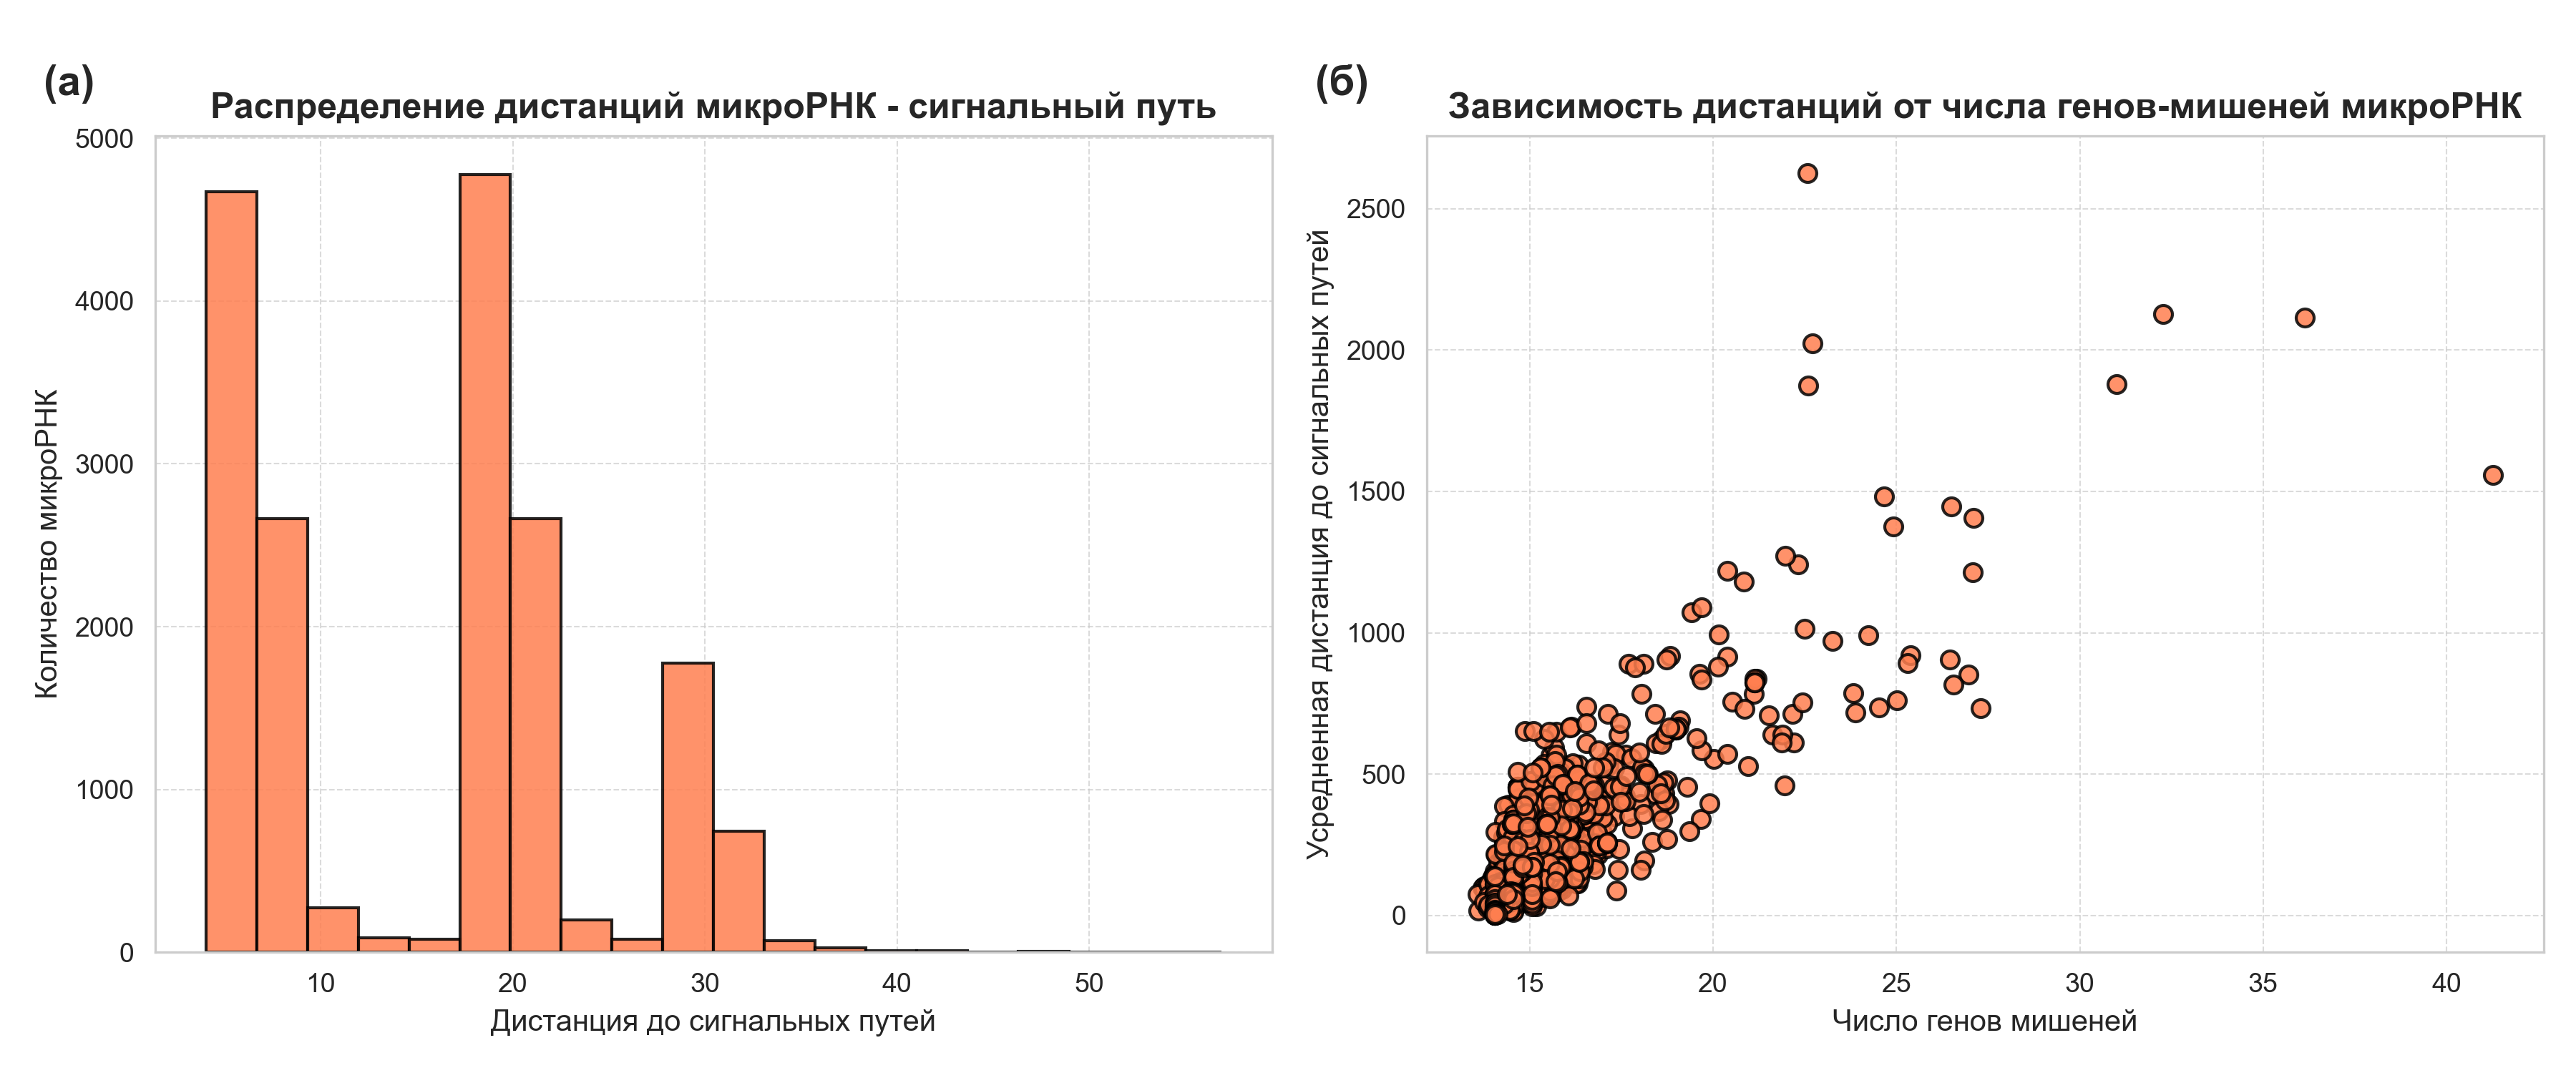
\includegraphics[width=1\textwidth]{Figs/Figure1.png}  % путь к файлу
    \caption{Распределение микроРНК по среднему расстоянию до рассматриваемых сигнальных путей}
    \label{fig:dist_global_hist}
\end{figure}

Из рисунка \ref{fig:dist_global_hist}(б) видно, что средняя удаленность от исследуемых путей растет с увеличением числа генов-мишеней, что представляется логичным, т.к. неиспользуемые для регуляции гены-мишени в постановке оптимизационной задачи (\ref{eq:optim_task}) будут увеличивать дистанцию между микроРНК и сигнальным путем. С точки зрения экспериментальной биологии такая логика справедлива, т.к. чем на большее число звеньев может влиять микроРНК - тем сильнее распределяется её влияние по всей системе, в то же время, исследовательский интерес представляет регуляция конкретных звеньев.

Уровень отсечки по дистанции $\tau$ искали как точку первого скачка эмпирической функции распределения (описано в методах):

\begin{figure}[H]
    \centering
    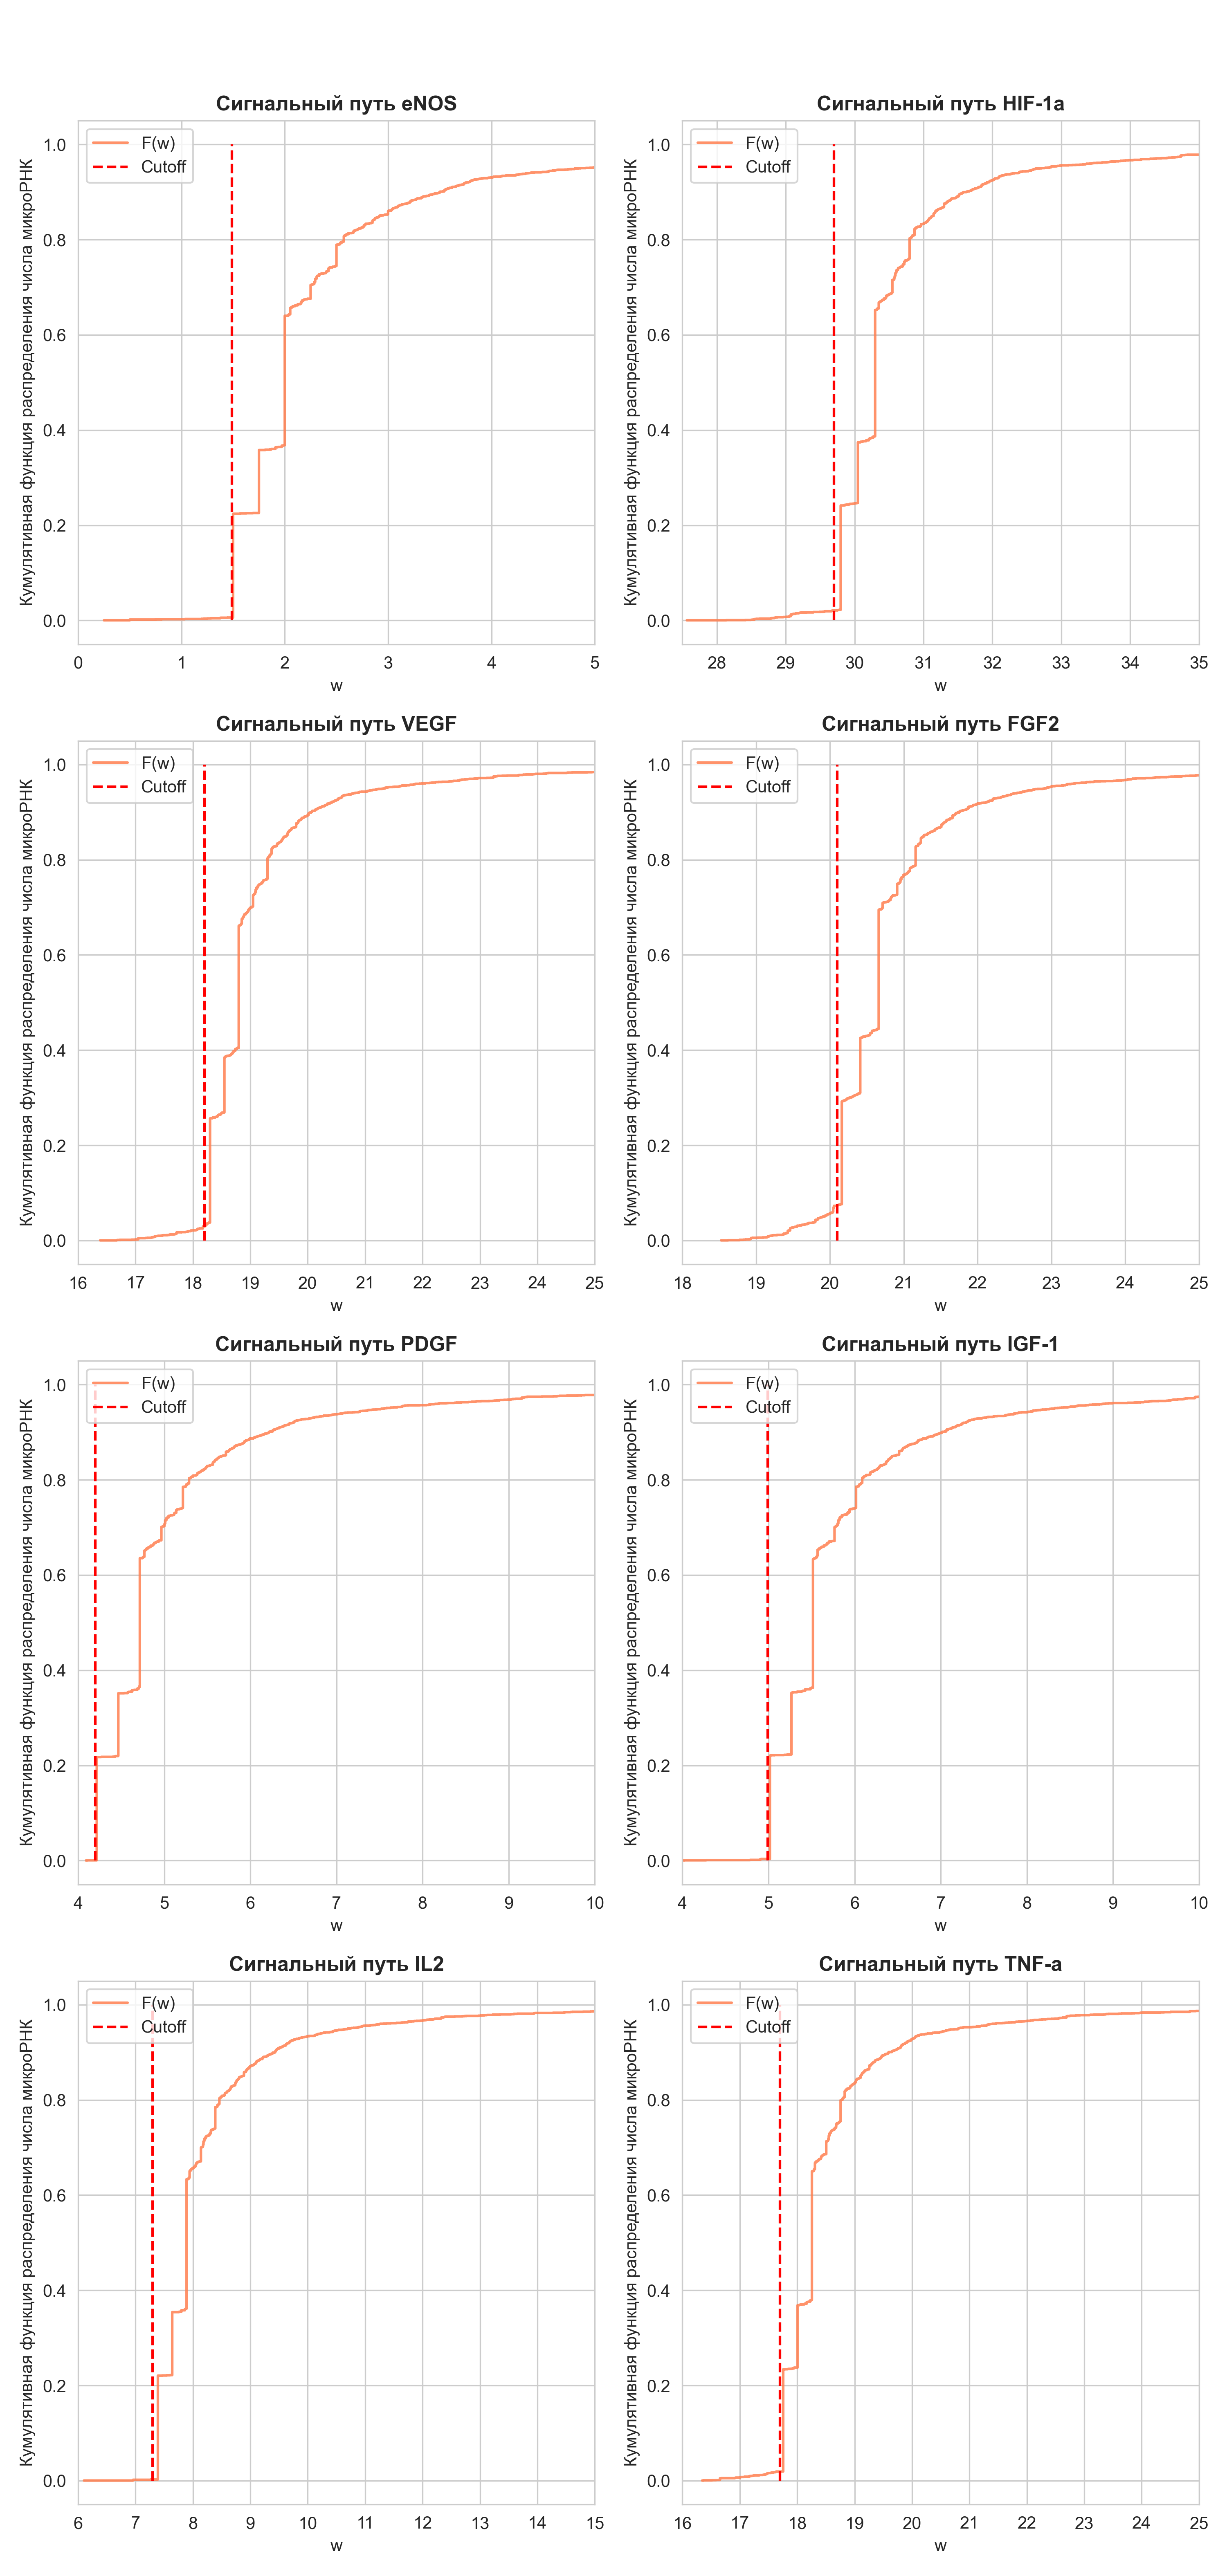
\includegraphics[width=1\textwidth, height=0.95\textheight]{Figs/Figure3.png}  % путь к файлу
    \caption{Распределение микроРНК по расстоянию до рассматриваемых сигнальных путей}
    \label{fig:dist_local_hist}
\end{figure}

МикроРНК удовлетворяющие условию $dist < \tau$ приведены в таблице \ref{tab:mirna_pathways}:

\begin{table}[ht]
    \centering
    \caption{Взаимосвязь микроRNA с изучаемыми сигнальными путями}
    \label{tab:mirna_pathways}
    \begin{adjustbox}{max width=1\textwidth}
    \begin{tabular}{p{3cm}lll}
    \toprule
    \textbf{Сигнальный путь} & \textbf{микроРНК (n мишеней)} & \textbf{Дистанция} & \textbf{Гены-мишени пути} \\
    \midrule
    
    \multirow{7}{*}{HIF-1a} & miR-301a-3p (395) & 29.4 & \{\textit{UBC}, \textit{UBB}, \textit{RPS27A}\} \\
     & miR-147a (149) & 29.07 & \{\textit{PSMA3}, \textit{VEGFA}, \textit{HIF3A}\} \\
     & miR-301b-3p (375) & 29.22 & \{\textit{UBC}, \textit{UBB}, \textit{RPS27A}\} \\
     & miR-454-3p (396) & 29.19 & \{\textit{UBC}, \textit{UBB}, \textit{RPS27A}\} \\
     & miR-4295 (366) & 29.14 & \{\textit{UBC}, \textit{UBB}, \textit{RPS27A}\} \\
     & miR-3666 (364) & 29.14 & \{\textit{UBC}, \textit{UBB}, \textit{RPS27A}\} \\
     & miR-653-5p (76) & 27.56 & \{\textit{UBC}, \textit{SEM1}, \textit{RPS27A}\} \\
    \midrule
    
    \multirow{2}{*}{VEGF} & miR-374b-5p (234) & 17.28 & \{\textit{AKT1}, \textit{NRP2}, \textit{PRKCD}, \textit{VEGFA}, \textit{RAC1}\} \\
     & miR-369-3p (163) & 17.45 & \{\textit{NRP2}, \textit{PRKCD}, \textit{VEGFA}, \textit{RAC1}, \textit{PLCG1}\} \\
    \midrule
    
    \multirow{3}{*}{FGF2} & miR-3652 (397) & 18.77 & \{\textit{GTF2F1}, \textit{POLR2D}, \textit{POLR2E}, \textit{MAPK1}\} \\
     & miR-4430 (397) & 18.77 & \{\textit{GTF2F1}, \textit{POLR2D}, \textit{POLR2E}, \textit{MAPK1}\} \\
     & miR-6134 (360) & 19.43 & \{\textit{GTF2F1}, \textit{FGFR1}, \textit{POLR2E}, \textit{FGF19}\} \\
    \midrule
    
    \multirow{2}{*}{PDGF} & miR-155-3p (68) & 4.09 & \{\textit{PLCG1}\} \\
     & miR-196b-3p (16) & 4.1 & \{\textit{SOS1}\} \\
    \midrule
    
    \multirow{2}{*}{IGF-1} & miR-2117 (57) & 4.79 & \{\textit{PIK3CB}, \textit{PDPK1}\} \\
     & miR-3191-5p (94) & 4.9 & \{\textit{IGF1R}, \textit{PDPK1}\} \\
    \midrule
    
    \multirow{7}{*}{IL2} & miR-422a (45) & 6.96 & \{\textit{PIK3CA}\} \\
     & miR-135a-5p (94) & 6.95 & \{\textit{JAK2}\} \\
     & miR-196b-3p (16) & 6.1 & \{\textit{SOS1}\} \\
     & miR-490-5p (41) & 6.96 & \{\textit{PIK3CA}\} \\
     & miR-6507-5p (132) & 7.26 & \{\textit{GAB2}\} \\
     & miR-2117 (57) & 6.96 & \{\textit{PIK3CB}\} \\
     & miR-1207-3p (84) & 7.29 & \{\textit{PIK3CB}\} \\
    \midrule
    
    \multirow{5}{*}{TNF-a} & miR-23a-3p (249) & 17.44 & \{\textit{ADAM17}, \textit{CHUK}, \textit{TNFAIP3}, \textit{XIAP}\} \\
     & miR-301b-3p (375) & 17.64 & \{\textit{UBC}, \textit{UBB}, \textit{XIAP}, \textit{RPS27A}\} \\
     & miR-454-3p (396) & 17.62 & \{\textit{UBC}, \textit{UBB}, \textit{XIAP}, \textit{RPS27A}\} \\
     & miR-4295 (366) & 17.55 & \{\textit{UBC}, \textit{UBB}, \textit{XIAP}, \textit{RPS27A}\} \\
     & miR-3666 (364) & 17.55 & \{\textit{UBC}, \textit{UBB}, \textit{XIAP}, \textit{RPS27A}\} \\
    \bottomrule
    \end{tabular}
    \end{adjustbox}
    \end{table}

Рассматривая приведенную таблицу с позиции решения задачи лексикографической оптимизации, можно обнаружить следующее:

Для сигнального пути HIF-1a наибольший интерес представляет miR651-5p, в силу наименьшей дистанции. Однако, наименьшая дистанция у этой микроРНК получилась из-за малого количества генов мишеней, а следовательно и штрафа $\beta$ (уравнение \ref{eq:optim_task}). С точки зрения же биологии и состава генов-мишеней - наибольший интерес представляет miR-147a, так как среди списка её мишеней присутствует \textit{HIF3A}. В любом случае, обе эти микроРНК заслуживают дальнейшего изучения с точки зрения их роли в регуляции сигнального пути HIF-1a в миокарде.

Для сигнального пути VEGF аналогичный анализ выявил две микроРНК: miR-374b-5p и miR-369-3p. Обе эти микроРНК имеют релевантный список генов-мишеней. Также обращает внимание, что при большем числе генов-мишеней у miR-374b она имеет меньшую дистанцию в сравнении с miR-369, что говорит о большем числе центральных генов среди генов-мишеней.

Для сигнального пути FGF2 две микроРНК (miR-3652 и miR-4430) имеют одинаково минимальную дистанцию при одинаковом списке генов-мишеней, входящих в сигнальный путь FGF2. Однако, в список мишеней miR-6134 входит \textit{FGFR1} и \textit{FGF19}.

Для сигнального пути TNF-a miR-23a-3p обладает и наименьшей дистанцией и в список её генов-мишеней входит ген \textit{TNFAIP3}.

Для сигнальных путей IGF-1, IL2, PDGF остается выбрить микроРНК из только по наименьшей дистанции: miR-2117, miR-196b-3p и miR-155-3p соответственно.